\section{A secure cloud storage system: Bdrive}
\todo[inline]{	
	* How does rekeying in bdrive work currently?\\
	* What security targets are covered\\
	* What is adventagous \\
	* Waht is disadventagous
	}
In the following we will describe the encryption scheme currently enrolled in Bdrive and give a rough overview of the existing solutions in the attribute-based encryption domain.

\subsection{Background}
\begin{figure*}[!ht]
\centering
    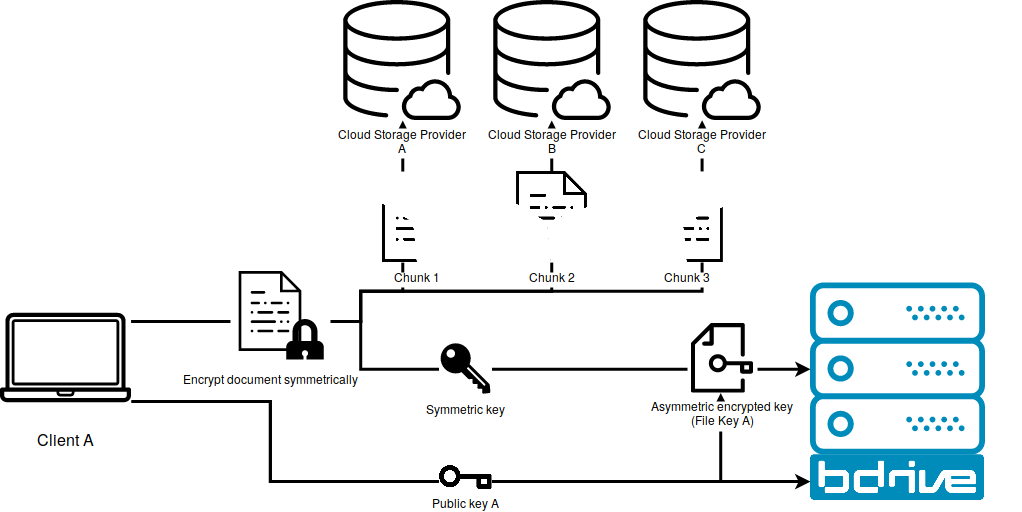
\includegraphics[width=0.8\linewidth]{img/bdrive1.png}\par 
    \caption{Client uploads an encrypted file to the CSPs and the file key and public key to Bdrive.}
    \label{fig:filekey}
\end{figure*}
\begin{figure*}[!ht]
\centering
    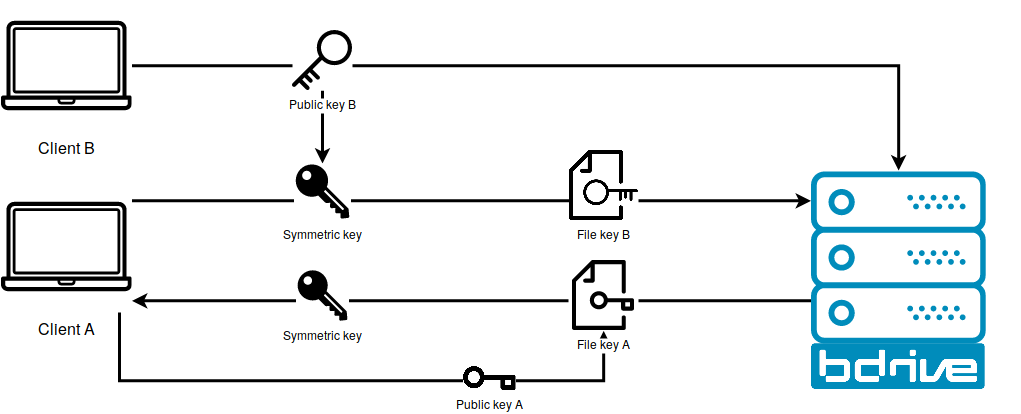
\includegraphics[width=0.8\linewidth]{img/bdrive2.png}\par
    \caption{Client A grants Client B access to the uploaded file by re-keying the file key}
    \label{fig:rekey}
\end{figure*}

Bdrive is a secure cloud storage which splits up files in smaller chunks that are saved separately on different cloud storage provider (CSP). To ensure end-to-end encryption a Bdrive client encrypts locally each of its chunks with a one-time symmetric key that is then encrypted under its own public key. This encrypted key is called a file key and it is uploaded to the Bdrive server where it is stored securely (see figure \ref{fig:filekey}).

Since each device of the same user has a different private-public key pair, the device is in charge of making the file keys accessible for a new device. This will be done by downloading each file key for the respective file, receiving the public key of the new device, decrypting the file key with its own private key, encrypting it again with the public key of the new device and finally, uploading the new file key to the Bdrive server. This process will be called re-keying (see figure \ref{fig:rekey}).

The number of file keys, that need to be maintained in Bdrive, grows linearly with the number of devices. In addition Bdrive allows to share files between different users. For each device of each user involved in a share a new file key has to be created and maintained. 

%The formula \ref{eq:rekey} describes the number of file keys Bdrive that need to be stored for each shared files between $U$ users, where each user $u_{i \in U}$ has $u_d$ devices.

%\begin{equation}
%n = \sum_{i}{d_i}
%\label{eq:rekey} 
%\end{equation}

%Lets construct an example where the manager of a company wants to create a shared folder with all company employees. It is a medium sized company with $50$ employees. Lets assume that at least haft of them have two Bdrive clients running. The manager wants to upload the $250$ photos of the last company trip.
%We end up by computing $3/2 * 50 * 250 = 18750$ file keys and for every new file uploaded $75$ new file keys need to be uploaded. 

\section{Bdrive Rekeying scheme}
\todo[inline]{find better title}

In Bdrive each device of a user generates a new RSA key pair on registaion. The fingerprint (hash) of the public key identifies the device uniquly. To save a file in the cloud the device fist encrypes the file symmetrically with the so called "filekey". The filekey equals the hash of the plain file content and so ensures tamperproofness and integirty on decryption. Since Bdrives supports end-to-end encryption the server should never be able to decrypt the file by itself. So the device encrypts the filekey asymmetrically with its own public key and uploads the filekey to the Bdrive server were it is stored securly. The encrypted file is uploaded to the different cloud storage provider. 

If the user wants to access a file locally, the devices requests the encrypted filekey from the server, downloads the file chunks from the cloud storage providers, decrypts the file key with his privat key and finally decrypts the file with the filekey. 

So far we saw how the encryption process is handled for a single device. However, this process turns out to be much more complex in computation in a multible devices setting.  If a user registers more then one device the exisiting data needs to be syncronized to the new device. The server nodifies the existing device for the new registered device and the public key of the new device is downloaded. Now, each filekey for each file of the user needs to be downloaded from the server and decrypted. To make them accessable for the new devices, they are encrypted with the new devices public key and uploaded again to the server. The new device can now start to download and decrypt the filekeys as decibed previously. 

Some may notice, that this approach is not scalable for a large number of devices. Others may argue that a user never has so many devices that this process is no longer maintanable. But a cloud storage system provides the possibility to share the files with other users. Which means that each device of the user that accepts the invitation to the share needs to have an own encrypted file key. This process scales with $O(n * f)$ keys. Were $n$ donates the number of devices onvolved in the sharing and $f$ the number of file versions in the share.\footnote{Each file consit of many file versions. Each file version needs an own file key since the content changes each time the file is updated.} Futher, we need to send $O(n * f)$ messages to send each device its personal filekey and we need to encrypt each filekey $n$ times which also results in $O(n * f)$ encryptions in total. 

If a new devices joins the share we need to make the existing file keys avaiable to the new devices which results in $O(f)$ additional encryptions, messages and keys. However, a big adventage of this scheme is that we don't have to anything if a member leaves the group. We simply remove all the filekeys belonging to the left device and do not further encrypt new uploaded files for this device. Forward secrey\footnote{Forward Secrecy: The left member do not have any knowledge about future shared content.} is ensured. Backwards secrecy is also provided since a device needs to rekey for the newly joined member to make the files accessable for him. 

How can we do better then this while still maintaining the same level of security? 